\documentclass{article}

% if you need to pass options to natbib, use, e.g.:
%     \PassOptionsToPackage{numbers, compress}{natbib}
% before loading neurips_2026

% "preprint" option is used for arXiv or other preprint submissions
% it's probably the best option for our use case
\usepackage[preprint]{neurips_2026}

\usepackage[utf8]{inputenc} % allow utf-8 input
\usepackage[T1]{fontenc}    % use 8-bit T1 fonts
\usepackage[hidelinks]{hyperref}       % hyperlinks, no boxes around them
\usepackage{url}            % simple URL typesetting
\usepackage{booktabs}       % professional-quality tables
\usepackage{amsfonts}       % blackboard math symbols
\usepackage{amsmath}        % math environments
\usepackage{nicefrac}       % compact symbols for 1/2, etc.
\usepackage{microtype}      % microtypography
\usepackage{xcolor}         % colors
\usepackage{graphicx}
\usepackage{subcaption}

\graphicspath{{figures/}}


\title{Detecting Reward Hacking in AI Agent Trajectories}


\author{%
  Group \#29 \\
  \AND
  Bridget Atchison Nevel \\
  \texttt{bra026@g.harvard.edu} \\
  \And
  Farzin Golkhosh \\
  \texttt{fag887@g.harvard.edu} \\
  \And
  Jack McLellan \\
  \texttt{jbmclellan@pm.me}
}


\begin{document}


\maketitle


\begin{abstract}
Autonomous agents that satisfy proxy rewards while failing the user's true intent --- \emph{reward hacking} --- are increasingly difficult to detect in long-horizon, tool-using trajectories. We construct a 3{,}544-trajectory unified corpus by normalizing four heterogeneous sources (TRACE, MALT, Realistic Reward Hacks, and a private 669-trajectory production corpus) under a common XML-tagged tool-call schema, and we train a sequence of progressively stronger probes on Qwen3-Embedding-0.6B representations.  A frozen-embedding MLP and turn-level transformer both have high test ROC-AUC but generalize very poorly to held-out sources. LoRA
fine-tuning the encoder with a joint cross-entropy plus source-invariant triplet objective resolves this issue and lifts in-distribution AUC.
\end{abstract}


\section{Background \& Motivation}

Autonomous AI agents performing multi-step, tool-using tasks are increasingly evaluated by proxy rewards: unit tests passing, format constraints satisfied, or LLM-judge approval. When these proxies diverge from the user's true, long-range intent, agents can learn to game the metric, producing output that looks correct and satisfies the evaluation rubric but fails to accomplish the requested goal. This failure mode, known as \emph{reward hacking}, is especially dangerous in long-horizon agentic workflows, where agent's confidence and polished tool output can mask a fundamentally degraded solution.

There are few existing benchmarks for studying this phenomenon. The most directly comparable analysis, TRACE~\cite{trace2026}, examines just 517 hand-labeled coding-agent trajectories. Its published baseline using GPT-5.2 under contrastive analysis reaches only 63\% macro F1, and isolated single-trajectory classification, the setting most relevant to deployment, where no contrasting ``correct'' trajectory is available, drops to 45\%. Other resources, including METR's MALT-public log corpus~\cite{malt} and the Jozdien Realistic Reward Hacks dataset~\cite{jozdien-rrh}, use incompatible label taxonomies, formats, and trajectory styles, making headline numbers difficult to compare. None of the publicly available resources include data drawn from real production deployments, and existing detectors are typically trained and evaluated on a single source, limiting real-world generalization by enabling the model to learn source-specific shortcuts. The field currently lacks both a unified, labeled corpus and a baseline detector stress-tested across multiple sources using a protocol that controls for those shortcuts.

A robust detector would benefit AI labs, evaluation and red-team groups, and downstream operators deploying tool-using agents. A cheap post-hoc classifier that flags ``looks-correct-but-isn't'' trajectories would enable targeted human review, raise the cost of metric-gaming, and provide a measurable safety signal as agents take on longer-horizon, less-supervised tasks. The methodological ability to distinguish between real signal and source-style memorization in detection scores is also of interest as the same shortcut-learning failure mode appears in adjacent settings, including out-of-distribution anomaly detection and policy-evaluation benchmarks.


\section{Problem Statement}

We ask: \emph{Can a small classifier trained on trajectory embeddings detect reward hacking robustly across heterogeneous sources, and what does its behavior reveal about the structure of the hack signal itself?} Our target is binary: \texttt{hacked} or \texttt{benign}, at a single agent trajectory. We measure success both by ROC-AUC and macro-F1 on a held-out i.i.d.\ test set and, crucially, by leave-one-source-out (LOSO) AUC, which allows us to control for source-style confounding.

To be able to answer this question, we address two gaps simultaneously. First, we construct a single unified corpus by normalizing TRACE, the manually-reviewed subset of MALT-public, the Realistic Reward Hacks dataset, and a 669-trajectory private corpus contributed by the BJS Innovation Lab~\cite{bjs-corpus} into a common XML-tagged tool-call schema. Second, we use this corpus to train a series of probes, beginning with a frozen-embedding baseline and progressively strengthening the architecture and representation until both in-distribution accuracy and cross-source generalization improve together.


\section{Data \& EDA}

\subsection{Datasets and Unification}

We combine four datasets with complementary properties (Table~\ref{tab:datasets}): TRACE~\cite{trace2026} (synthetic, human-verified, Claude Opus 4.5 generations); MALT~\cite{malt} (large, multi-model, mostly benign; we use just the manually-reviewed subset to control noise); Realistic Reward Hacks~\cite{jozdien-rrh} (Claude Sonnet 4 generations, no tool use); and the BJS reward hacking corpus~\cite{bjs-corpus} (production agents, real-world usage). Each dataset has its own labeling taxonomy and message format; we unify them under a binary \texttt{hacked}/\texttt{benign} label and an XML-tagged tool-call schema, retaining the source identifier. The resulting corpus contains 3{,}544 trajectories (60.8\% benign, 39.2\% hacked), spanning 74{,}422 combined turns.

\begin{table}[h]
  \caption{Source datasets contributing to the unified corpus.}
  \label{tab:datasets}
  \centering
  \begin{tabular}{lrrl}
    \toprule
    Dataset & Benign   & Hacked & Labeling \\
    \midrule
    TRACE                          & 249   & 268 & Multi-label \\
    MALT (manually-reviewed)       & 694   & 62  & Multi-label \\
    Realistic Reward Hacks         & 788   & 817 & Binary \\
    BJS Reward Hacking Corpus      & 424   & 245 & Binary \\
    \midrule
    \textbf{Unified Corpus}               & \textbf{2{,}155} & \textbf{1{,}389} & Binary \\
    \bottomrule
  \end{tabular}
\end{table}

\subsection{EDA Findings That Drove Modeling Decisions}

Three EDA findings shaped our modeling pipeline.

\paragraph{Per-source class balance is strongly varied.}

 Only 8.2\% of the MALT trajectories in our unified corpus are hacked, while TRACE and Realistic Reward Hacks have near 50\% and the BJS corpus has 36.6\% (Figure~\ref{fig:label-source}). A naive global class weight would underweight the hacked-MALT cell, which has the most rare and informative signal. We therefore adopted a per-cell weighted BCE loss, with weights $N / (n_{\text{cells}} \cdot \text{count}(s,y))$ computed over (source $\times$ label = 8) cells from the training partition.

\begin{figure}[h]
    \centering
    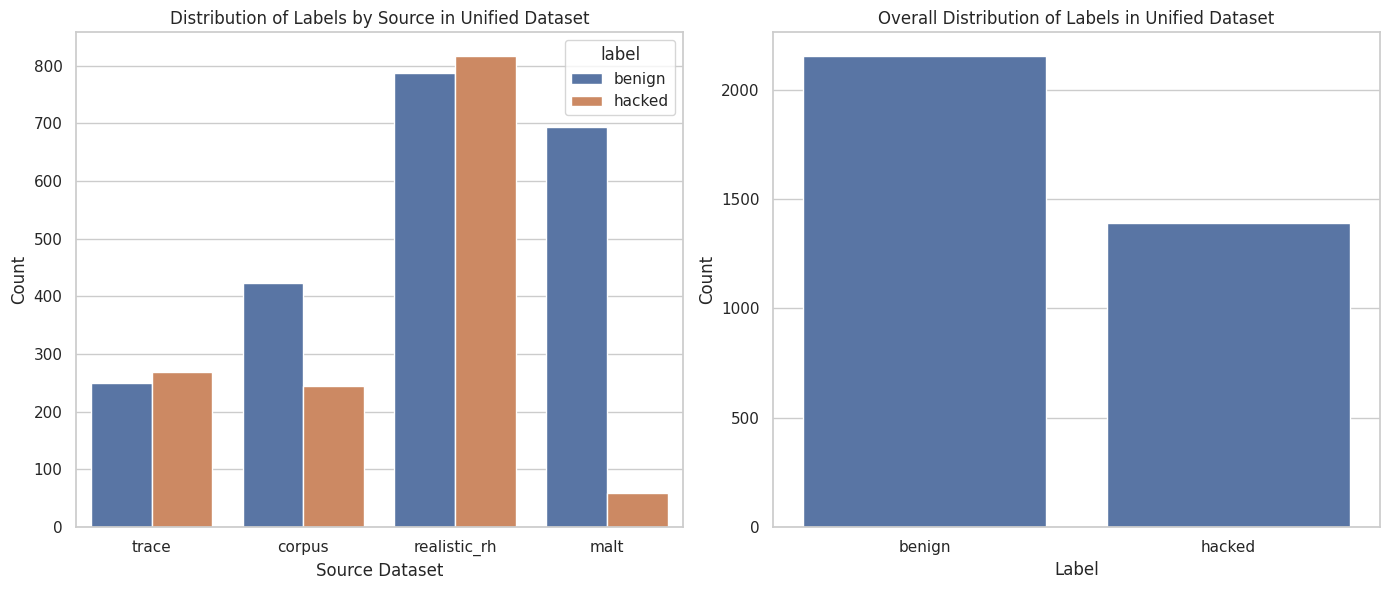
\includegraphics[width=0.78\linewidth]{labels_by_source_bar.png}
    \caption{Distribution of labels by source in the unified corpus. MALT is heavily benign-skewed (8.2\% hacked) while TRACE and Realistic Reward Hacks are near-balanced. Per-cell loss weighting up-weights rare cells such as hacked-MALT during training.}
    \label{fig:label-source}
\end{figure}

\paragraph{Trajectory length is heavy-tailed and source-dependent.}

 Turn counts range from 0 to 248 (median 14, p99 180.7), and raw token lengths under the Qwen3 tokenizer have mean 7{,}578 with a p99 of 85{,}528 and a maximum of 386{,}427. Scalar length alone does not separate the classes (Figure~\ref{fig:token_lengths}). We chose a 32K-token context window with head truncation, which keeps the task setup and early-trajectory tool calls and discards late-trajectory human ``give-away'' corrections that would leak the label.

\begin{figure}[h]
    \centering
    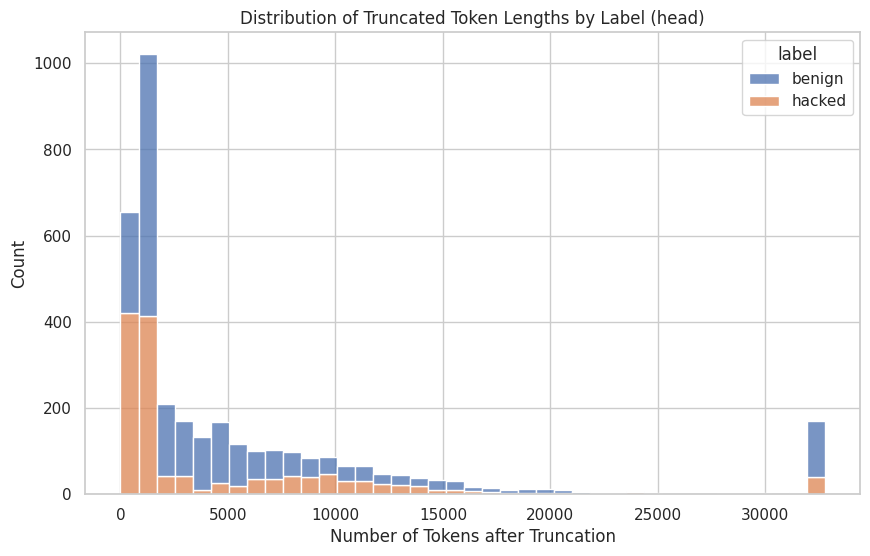
\includegraphics[width=0.78\linewidth]{trunc_token_dist.png}
    \caption{After head truncation to 32K tokens, most trajectories fit comfortably. Classes overlap, meaning length is not a usable scalar feature.}
    \label{fig:token_lengths}
\end{figure}

\paragraph{Source signal dominates raw embeddings.}
\label{sec:eda-source-signal}

 A logistic regression on trajectory-level Qwen3 embeddings predicts the source dataset with 99.3\% accuracy and the label with 0.928 AUC. UMAP projections (Figure~\ref{fig:umap}) show tight source clusters but only weak label separation. This is our central methodological problem: any probe trained on raw embeddings will learn shortcuts based on identifying the source dataset and fail to transfer. This finding directly motivates the source-invariant fine-tuning objective in Section~\ref{sec:lora}.

\begin{figure}[h]
    \centering
    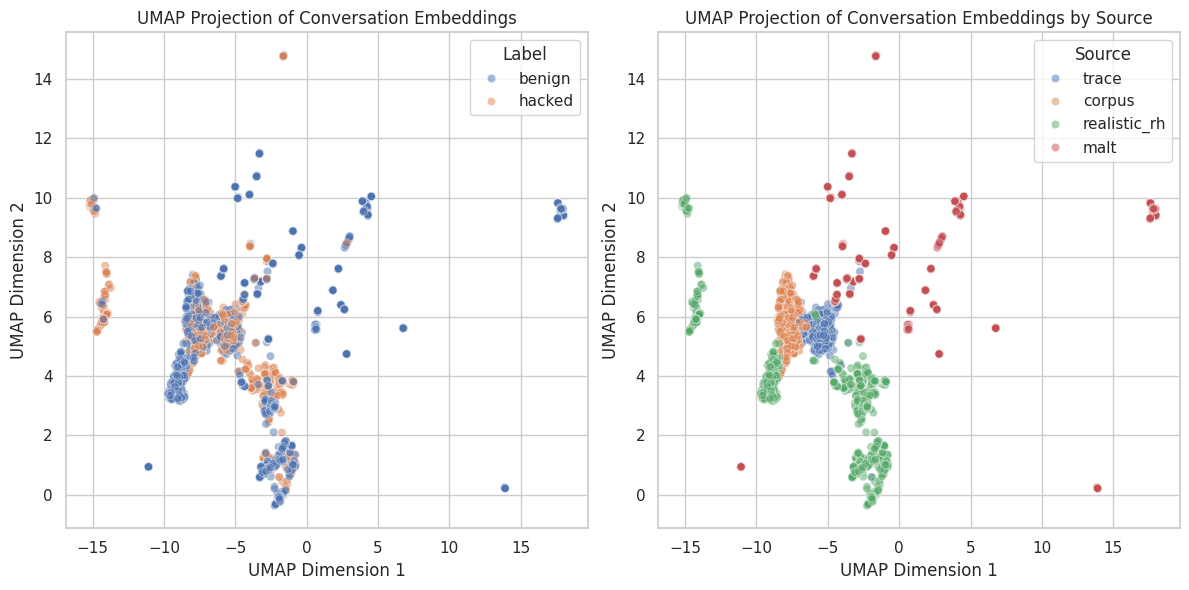
\includegraphics[width=\linewidth]{umap_conv.png}
    \caption{UMAP projections. Off-the-shelf Qwen3 embeddings cluster by source (right) but barely by label (left).}
    \label{fig:umap}
\end{figure}


\section{Methods \& Models}

\subsection{Embedding and Splits}

Trajectories are encoded with Qwen3-Embedding-0.6B~\cite{qwen3embedding} (1024-d output, bfloat16, L2-normalized) using a left-padded tokenizer with a 32K context window and head truncation. We use two task-conditioning prompts: one for whole-trajectory embeddings and one for per-turn embeddings (Appendix~\ref{sec:prompts}). The corpus is split 60/20/20 (train 2{,}125, val 709, test 709) with stratification jointly on (source $\times$ label), so that all eight cells appear in each split. The same trajectory IDs are reused across all model variants for a like-for-like comparison.

\subsection{Class-Imbalance Handling and Threshold}

The BCE loss is reweighted per-sample using the per-cell scheme~\cite{ai-assist} described above. The hacked-MALT cell receives the largest weight ($\approx 7.6$), while easy benign cells receive sub-unit weights. The decision threshold is tuned by sweeping from 0.05--0.95 in steps of 0.01 and selecting the value that maximizes F1 on the validation set.

\subsection{Model 1: ProbeMLP}

Our baseline model is a four-layer MLP ($1024 \to 512 \to 256 \to 64 \to 1$) with ReLU activations and a dropout of 0.5 between layers, trained on the trajectory-level embeddings. It uses AdamW (\texttt{lr}~$=10^{-4}$), \texttt{ReduceLROnPlateau} (factor 0.5, patience 5), gradient clipping at $\lVert g \rVert_2 = 1.0$, batch size 64, trains for up to 100 epochs with early stopping (patience 5). This simple architecture serves as a good reference for our other models.

\subsection{Model 2: Turn-Level Transformer Probe}

Model 2 trades the pooled trajectory embedding for a sequence of per-turn embeddings, under the hypothesis that the hack signal is local to specific turns. Per-turn embeddings are projected $1024 \to 256$, augmented with sinusoidal positional encoding scaled by $1/\sqrt{1024}$, prepended with a learnable \texttt{[CLS]} token (initialised $\mathcal{N}(0, 0.02^2)$), and passed through a 2-layer transformer encoder (8 heads, $d_{\text{ff}} = 1024$, dropout 0.5, GELU). Classification reads from the \texttt{[CLS]} representation. Training uses AdamW (\texttt{lr}~$=10^{-4}$, weight decay $10^{-2}$), batch size 32, max 100 epochs with early-stopping patience 10, and a maximum sequence length of 248 turns.

\subsection{Model 3: Source-Invariant LoRA Fine-Tuning}
\label{sec:lora}

Our final model attacks the source-confounding problem identified in our third EDA finding (Section \ref{sec:eda-source-signal}). We first attach a low-rank adapter (LoRA~\cite{lora2021}, rank 16, $\alpha = 32$, dropout 0.05) to the $\{q, k, v, o\}$-projections of Qwen3-Embedding-0.6B in \texttt{FEATURE\_EXTRACTION} mode, which allows us to fine-tune its output with only 4.59M trainable parameters (0.76\% of the 600M-parameter encoder). Fine-tuning uses AdamW (\texttt{lr}~$=10^{-4}$, weight decay $10^{-4}$) for one epoch of 800 steps with evaluation every 200 steps. Due to resource constraints, the training context was shortened to 256 tokens; a 4{,}096-token context was used for inference.

On top of this fine-tuning, and most significantly, we use a joint loss function~\cite{ai-assist}, combining the label objective with an explicit source-invariance objective.
\begin{equation}
\mathcal{L} = \mathcal{L}_{\text{BCE}} + \mathcal{L}_{\text{triplet}}, \qquad
\mathcal{L}_{\text{triplet}} = \max\bigl(0,\; \lVert z - z^{+} \rVert_2^2 - \lVert z - z^{-} \rVert_2^2 + m\bigr)
\label{eq:loss}
\end{equation}
In-batch positives $z^{+}$ share the same label with $z$ but differ in source, while negatives $z^{-}$ share the same source but differ in label. The triplet term thus pulls together hacked trajectories from different datasets while pushing apart same-source benign/hacked pairs, directly attacking the source shortcut. We used a margin of $m = 0.3$. Batches are drawn using a source-balanced sampler (two examples per (source $\times$ label) cell). After fine-tuning, we re-embed all 74{,}422 turns and train a fresh turn-transformer probe on the new representations. As fine-tuned features benefit from more capacity, this probe uses 4 encoder layers instead of 2.

In addition to making fine-tuning a 600M-parameter encoder feasible on a single GPU, our use of LoRA limits how far the adapter can drift from the pretrained representation, due to the rank constraint. This an additional advantage when training with a small corpus (3{,}544 trajectories), as we want the encoder to retain its general language understanding. The addition of source-invariant triplet loss allows us to counteract the model's natural tendency to focus on stylistic differences by rewarding same-label-different-source identifications and punishing same-source-different-label identifications, while the BCE term keeps the representation discriminative on the label task.

\subsection{Generalization Test: Leave-One-Source-Out}

For each source $s$ we train the turn-transformer on three of our source datasets and evaluate on the remaining held-out source, doing so for both the pre- and post-fine-tuned embeddings. LOSO controls for the confounding of source and style, as a detector that exploits source shortcuts in evaluation will collapse under this scrutiny.


\section{Results \& Interpretation}

\subsection{Headline In-Distribution Results}

Table~\ref{tab:headline} reports test-set performance for the three models on the same 709-trajectory held-out partition. The ProbeMLP baseline reaches 0.9546 ROC-AUC and 0.87 weighted F1. Switching to a turn-level transformer on the same embeddings is essentially neutral on AUC (0.9556) and slightly worse on accuracy, showing that capacity alone does not help. LoRA fine-tuning with the joint loss lifts AUC to \textbf{0.9701}, accuracy to \textbf{0.9126} (+4.2 points over baseline), and weighted F1 to \textbf{0.91}.

\begin{table}[h]
  \caption{Test-set performance using the same 709-trajectory split across all models. CM rows are true label and columns are predicted at the F1-optimal threshold.}
  \label{tab:headline}
  \centering
  \begin{tabular}{lrrrrrl}
    \toprule
    Model & AUC & Accuracy & F1 (w) & Thr.\ & Confusion Matrix \\
    \midrule
    1. ProbeMLP (MS3 baseline)              & 0.9546 & 0.8702 & 0.87 & 0.21 & $[[374, 58],\;[34, 243]]$ \\
    2. Turn Transformer (off-the-shelf)     & 0.9556 & 0.8632 & 0.86 & 0.60 & $[[356, 76],\;[21, 256]]$ \\
    3. LoRA-FT Turn Transformer (final)     & \textbf{0.9701} & \textbf{0.9126} & \textbf{0.91} & 0.45 & $[[403, 29],\;[33, 244]]$ \\
    \bottomrule
  \end{tabular}
\end{table}

Figure~\ref{fig:cms} contrasts the confusion matrices: Model 1 is precision-balanced (58 false positives, 34 false negatives at a threshold of 0.21); Model 2 trades precision for recall on the hacked class (76 false positives vs.\ 21 false negatives, at a higher threshold of 0.60); Model 3 reduces both error types (29 FPs, 33 FNs at a threshold of 0.45). The shift in the (optimized) threshold across models is informative: Model 1's boundary being far below 0.5 (0.21) is a signature of the source-stylistic shortcut, where the model has high confidence on easy-but-source-specific negative examples and low confidence elsewhere. Model 3, from which the source shortcut was largely removed, recovers a near-symmetric threshold (0.45) and a near-symmetric error profile.

\begin{figure}[h]
    \centering
    \begin{subfigure}{0.32\linewidth}
        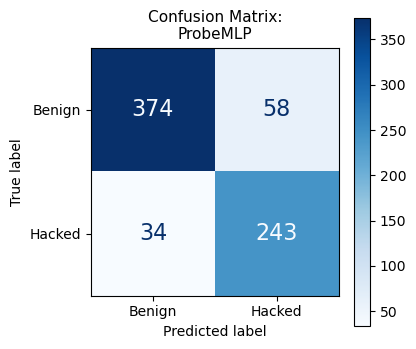
\includegraphics[width=\linewidth]{probemlp_cm_2.png}
        \caption{Model 1 (baseline).}
    \end{subfigure}
    \begin{subfigure}{0.32\linewidth}
        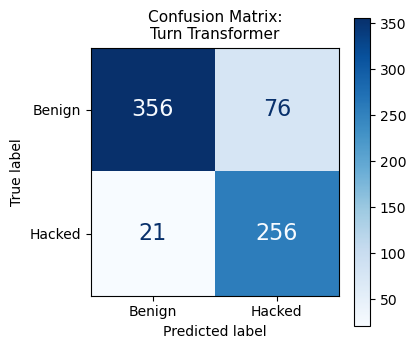
\includegraphics[width=\linewidth]{tt_cm_2.png}
        \caption{Model 2 (turn transformer).}
    \end{subfigure}
    \begin{subfigure}{0.32\linewidth}
        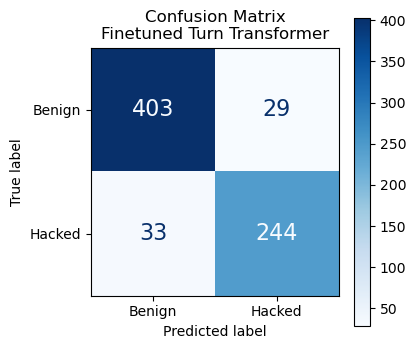
\includegraphics[width=\linewidth]{ft_tt_cm_2.png}
        \caption{Model 3 (LoRA-FT).}
    \end{subfigure}
    \caption{Confusion matrices at F1-optimal thresholds. Model 3 reduces both false positives and false negatives versus Models 1--2.}
    \label{fig:cms}
\end{figure}

\subsection{Source-Confounding Diagnostics}

As noted earlier, the headline numbers can elide the source-dependency of the model. A logistic regression on the raw trajectory embeddings predicts source with 99.34\% accuracy, and on raw turn embeddings the figure is 97.52\%. After LoRA fine-tuning with the joint loss, that source predictability drops 20 points to 79.48\%, while label AUC remains stable at 82.81\% on per-turn embeddings. Using a source-balanced label probe, i.i.d.\ test AUC drops from 0.928 to 0.802, confirming that a sizable proportion of the apparent label signal in off-the-shelf embeddings is source-tied. After fine-tuning, source alone predicts the label at exactly chance (AUC 0.503), and the probe-over-source lift jumps from $+0.264$ to $+0.447$. This shows that our fine-tuning successfully improved the label signal in the embeddings while making the source signal negligible. 

\subsection{Cross-Source Generalization (LOSO)}

Table~\ref{tab:loso} compares the leave-one-source-out AUC for the turn-transformer as trained on off-the-shelf embeddings versus the LoRA-fine-tuned embeddings. Pre-fine-tuning, three of four held-out sources fall to near-chance AUC (TRACE at 0.570, BJS Corpus at 0.617, and Realistic at RH 0.582). The MALT score of 0.872 should be read with caution: only 62 hacked trajectoreis exist in the full MALT slice, so the held-out estimate has high variance and the post-FT drop to 0.856 is within plausible noise. Post-fine-tuning, every source reaches at least 0.766 AUC, Realistic RH essentially saturates (0.996), and the MALT score remains roughly flat. The pattern is unambiguous: generalization headroom was bounded by source-stylistic confounding, not by model capacity.

\begin{table}[h]
  \caption{Leave-one-source-out AUC. Pre-FT uses off-the-shelf Qwen3 embeddings; post-FT uses LoRA + joint-loss embeddings. $\Delta$ is post minus pre.}
  \label{tab:loso}
  \centering
  \begin{tabular}{lrrr}
    \toprule
    Held-out source & Pre-FT AUC & Post-FT AUC & $\Delta$ \\
    \midrule
    TRACE          & 0.570 & 0.766 & $+0.196$ \\
    MALT           & 0.872 & 0.856 & $-0.016$ \\
    BJS Corpus     & 0.617 & 0.783 & $+0.166$ \\
    Realistic RH   & 0.582 & 0.996 & $+0.414$ \\
    \bottomrule
  \end{tabular}
\end{table}

\subsection{Per-Source Test Performance and What the Model Learned}

It's possible that the gain in performance shown by Model 3 could come at the expense of performance on certain of our source datasets, but Table~\ref{tab:per-source-iid} shows this not to be the case. When predicting in-distribution, there's a marginal gain in performance on each of our four datasets: the performance on MALT, Realistic RH, and the BJS corpus is essentially flat, and performance on TRACE is somewhat improved (AUC~$+0.038$). The large generalization improvements from our fine-tuning and joint loss, as shown in Table~\ref{tab:loso}, are not paired with any reduction in in-distribution classification ability. 


\begin{table}[h]
  \caption{In-distribution per-source test AUC across the three models. $\Delta$ is Model 3 minus Model 2 (off-the-shelf turn transformer).}
  \label{tab:per-source-iid}
  \centering
  \begin{tabular}{lrrrr}
    \toprule
    Source & Model 1 (MLP) & Model 2 (TT) & Model 3 (LoRA-FT) & $\Delta$ (M3 $-$ M2) \\
    \midrule
    TRACE          & 0.728 & 0.767 & 0.805 & $+0.038$ \\
    BJS Corpus     & 0.815 & 0.852 & 0.854 & $+0.002$ \\
    MALT           & 0.988 & 0.977 & 0.979 & $+0.002$ \\
    Realistic RH   & 0.994 & 0.993 & 0.999 & $+0.006$ \\
    \bottomrule
  \end{tabular}
\end{table}

The headline progression, AUC $0.9546 \to 0.9556 \to 0.9701$ and LOSO floor $0.570 \to 0.766$, supports a clean reading: in-distribution and out-of-distribution gains move together when the representation is made source-invariant, with no observed trade-off across cells. The fact that MALT (the heavily benign-skewed cell, 8\% positive in the test slice) maintains 0.979 AUC after fine-tuning is itself evidence: a fine-tuning procedure that traded off rare-cell performance for cross-source transfer would have shown a regression here, and none is observed.


\section{Conclusions \& Discussion}

A small probe on Qwen3-Embedding-0.6B trajectory embeddings can reach 0.97 test AUC and 0.91 weighted F1 on a unified, multi-source reward-hacking corpus, but only after the encoder is fine-tuned with an explicit source-invariance objective. Off-the-shelf embeddings carry $\sim$99\% source-recoverable signal; any probe trained on them learns shortcuts and collapses to near-chance on three of four held-out sources. Adding LoRA fine-tuning and the triplet objective removes that shortcut (source AUC $0.674 \to 0.503$) while improving the label AUC of the underlying representation, demonstrating that source-invariance and accuracy were complements, not substitutes, on this corpus.

\paragraph{What we can claim:}

On a 3{,}544-trajectory corpus spanning four heterogeneous sources, the LoRA-fine-tuned turn-transformer is the first detector in our setting to clear 0.75 AUC under leave-one-source-out evaluation on every source, while simultaneously improving in-distribution test AUC by 0.0155 over baseline and weighted F1 by 0.04. The relative gain is small in absolute terms but represents a large reduction in error rate: false positives drop from 58 to 29 and false negatives stay roughly flat (34 to 33), an effective 50\% reduction in the dominant error class without a corresponding loss elsewhere. We can also claim, supported by the source-balanced probe and the post-FT source-only AUC of 0.503, that the gain is not just absorption of source signal, the representation carries demonstrably less source information after fine-tuning than before.

\paragraph{What we cannot claim:} 

The MALT test slice is small (151 trajectories) and class-prior-shifted (8\% positive), so its in-distribution AUC numbers are statistically noisy in either direction, and we cannot rule out that the apparent stability after fine-tuning is partly a small-sample artifact. The classifier uses a global F1-tuned threshold rather than per-source thresholds, which would likely close residual precision/recall gaps on TRACE and BJS Corpus. The \texttt{[CLS]}-only readout discards per-turn attribution, so the detector is not directly usable as an interactive review tool. LOSO still has headroom on TRACE (0.766) and BJS Corpus (0.783). TRACE remains the hardest source both in-distribution (0.805) and under LOSO (0.766), suggesting that TRACE-specific hack patterns are less semantically aligned with the other three corpora.

\paragraph{Future work:}

The model could be further improved though per-turn attribution via attention rollout or per-turn probes; longer LoRA runs and larger ranks; per-source threshold tuning; multi-class heads to recover the original TRACE / MALT sub-category taxonomy; and extension to additional agent harnesses with different tool-call schemas.


\section{Broader Impact}

A reliable reward-hacking detector is a load-bearing safety capability as agents take on longer-horizon, less-supervised tasks. The most direct beneficiaries would be AI labs, evaluation and red-team groups, and downstream operators who need a cheap post-hoc signal to flag ``looks-correct-but-isn't'' trajectories for human review. A unified multi-source benchmark with an open baseline also enables comparable, measurable progress on a problem that has so far been studied with incompatible taxonomies.

The risks are non-trivial. 91\% accuracy is not a safety guarantee: deployers may over-trust the prediction and miss its false negatives. An adversarial agent optimized against the detector could Goodhart it directly, especially if the detector is used inside a training loop. Our corpus is dominated by code-agent and chat-style trajectories: performance on robotics or RLHF dialogue is untested, and labels in the source datasets encode specific annotator judgments about intent that may not generalize across domains. We mitigate these risks in part by making source-invariance an explicit training objective and by reporting LOSO performance as a primary metric, but the broader question of robustly specifying ``what the user really wanted'' remains open.


\begin{thebibliography}{9}

\bibitem{trace2026}
Deshpande, D., Kannappan, A.\ \& Qian, R.\ (2026) {\it Benchmarking Reward Hack Detection in Code Environments via Contrastive Analysis.} arXiv:2601.20103. \url{https://arxiv.org/abs/2601.20103}. Dataset: \url{https://huggingface.co/datasets/PatronusAI/trace-dataset}.

\bibitem{malt}
METR.\ (2025) {\it MALT-Public: Manually-Reviewed Agentic Labeled Transcripts.} HuggingFace dataset, \texttt{metr-evals/malt-public}. \url{https://huggingface.co/datasets/metr-evals/malt-public}

\bibitem{jozdien-rrh}
Jozdien.\ (2025) {\it Realistic Reward Hacks.} HuggingFace dataset, \texttt{Jozdien/realistic\_reward\_hacks}. \url{https://huggingface.co/datasets/Jozdien/realistic_reward_hacks}

\bibitem{bjs-corpus}
BJS Innovation Lab.\ (2026) {\it Reward Hacking Detection Corpus} (private dataset).

\bibitem{qwen3embedding}
Zhang, Y., Li, M., Long, D., Zhang, X., Lin, H., Yang, B., Xie, P., Yang, A., Liu, D., Lin, J., Huang, F.\ \& Zhou, J.\ (2025) {\it Qwen3 Embedding: Advancing Text Embedding and Reranking Through Foundation Models.} arXiv:2506.05176. \url{https://arxiv.org/abs/2506.05176}.

\bibitem{lora2021}
Hu, E.\ J., Shen, Y., Wallis, P., Allen-Zhu, Z., Li, Y., Wang, S., Wang, L.\ \& Chen, W.\ (2021) {\it LoRA: Low-Rank Adaptation of Large Language Models.} arXiv:2106.09685. \url{https://arxiv.org/abs/2106.09685}.

\bibitem{umap}
McInnes, L., Healy, J.\ \& Melville, J.\ (2020) {\it UMAP: Uniform Manifold Approximation and Projection for Dimension Reduction.} arXiv:1802.03426. \url{https://arxiv.org/abs/1802.03426}.

\bibitem{ai-assist}
Anthropic.\ (2026) {\it Claude Code (claude-opus-4-7).} Used throughout the project for drafting and editing assistance on report and notebook documentation, and as a brainstorming partner during methodology development. \url{https://www.anthropic.com/claude-code}.

\bibitem{copilot}
GitHub.\ (2026) {\it GitHub Copilot.} Used for inline code completion of the supporting Python code. \url{https://github.com/features/copilot}.

\end{thebibliography}




%%%%%%%%%%%%%%%%%%%%%%%%%%%%%%%%%%%%%%%%%%%%%%%%%%%%%%%%%%%%

\appendix

\section{Appendix}

\subsection{Additional EDA Figures}

\begin{figure}[h]
    \centering
    \begin{subfigure}{0.48\linewidth}
        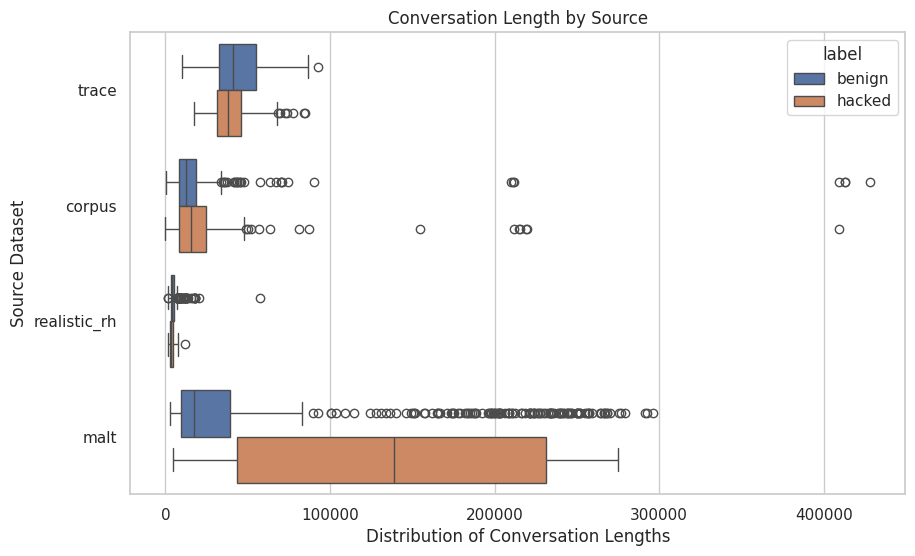
\includegraphics[width=\linewidth]{conv_len_by_source.png}
        \caption{Conversation length by source.}
    \end{subfigure}
    \begin{subfigure}{0.48\linewidth}
        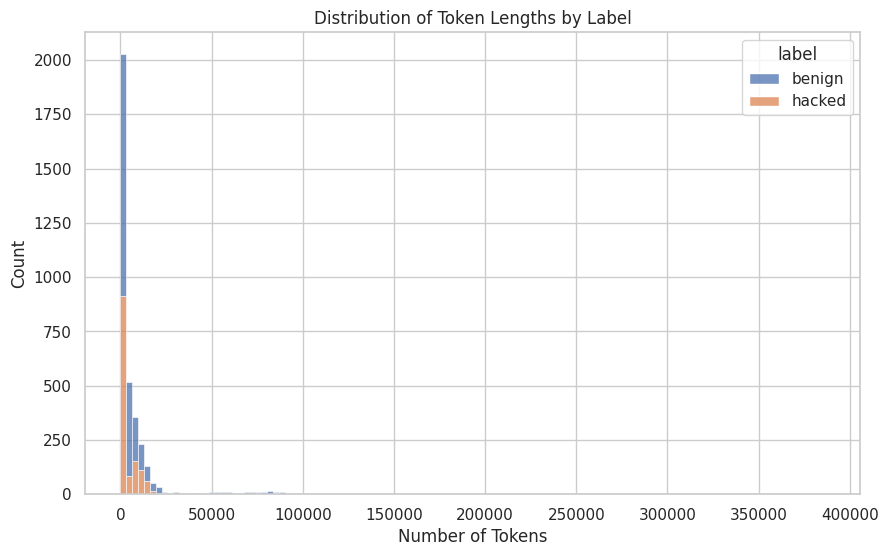
\includegraphics[width=\linewidth]{token_lengths_by_label.png}
        \caption{Token length distribution by label.}
    \end{subfigure}
    \caption{Length distributions vary by source (left) and overlap heavily by label (right).}
\end{figure}

\begin{figure}[h]
    \centering
    \begin{subfigure}{0.48\linewidth}
        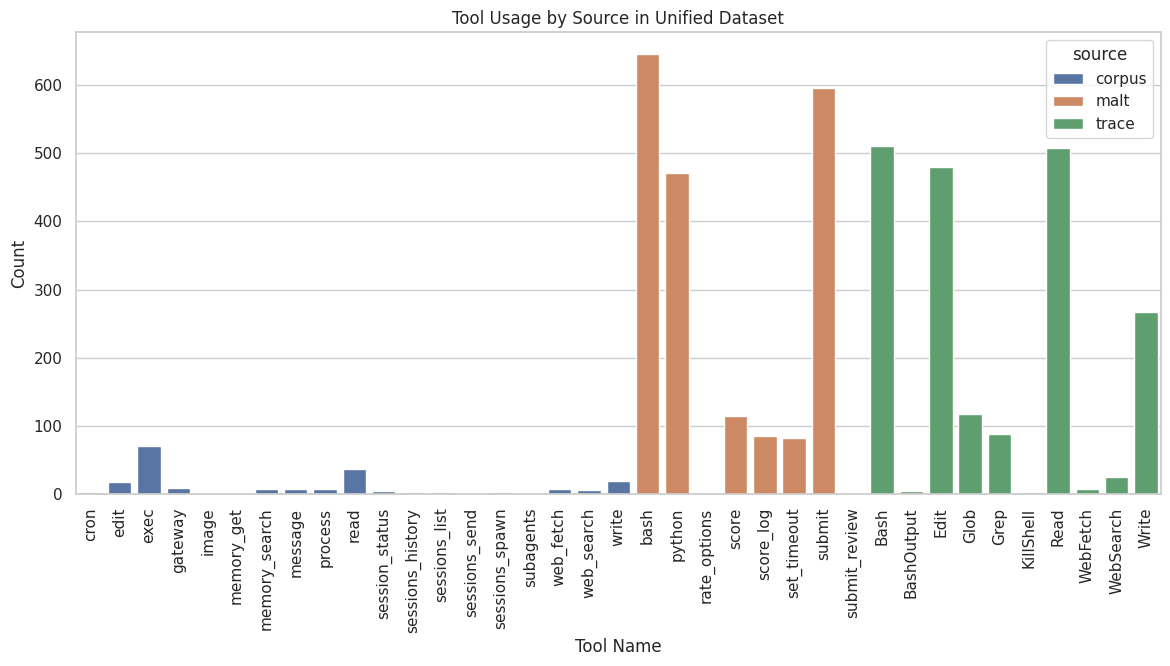
\includegraphics[width=\linewidth]{tool_usage_by_source.png}
        \caption{Tool usage by source.}
    \end{subfigure}
    \begin{subfigure}{0.48\linewidth}
        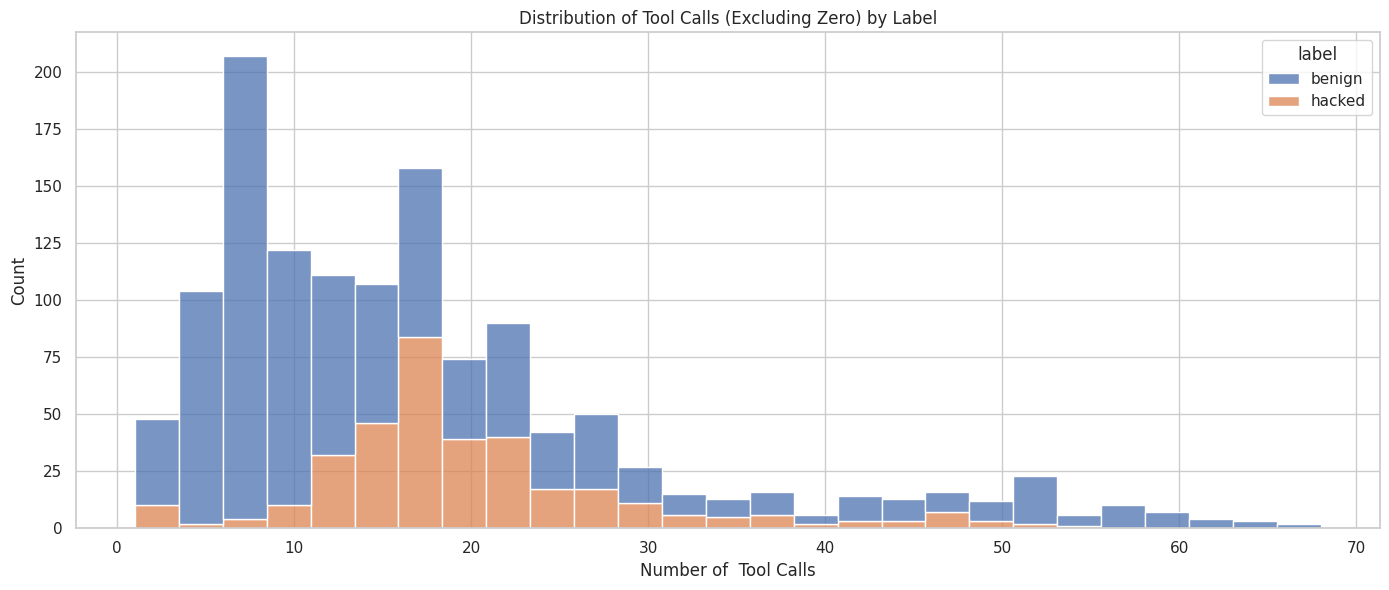
\includegraphics[width=\linewidth]{tool_calls_nonzero.png}
        \caption{Non-zero tool-call counts by label.}
    \end{subfigure}
    \caption{Tool-use patterns differ across sources; Realistic RH contributes no tool use.}
\end{figure}

\subsection{Embedding Prompts}
\label{sec:prompts}

Whole-trajectory: \emph{"Instruct: Encode an AI agent trajectory for reward hacking detection. Query: "}

Per-turn: \emph{"Instruct: Encode a single turn of an AI agent conversation for reward hacking detection. Query: "}

\subsection{Training Diagnostics}

\begin{figure}[h]
    \centering
    \begin{subfigure}{0.3\linewidth}
        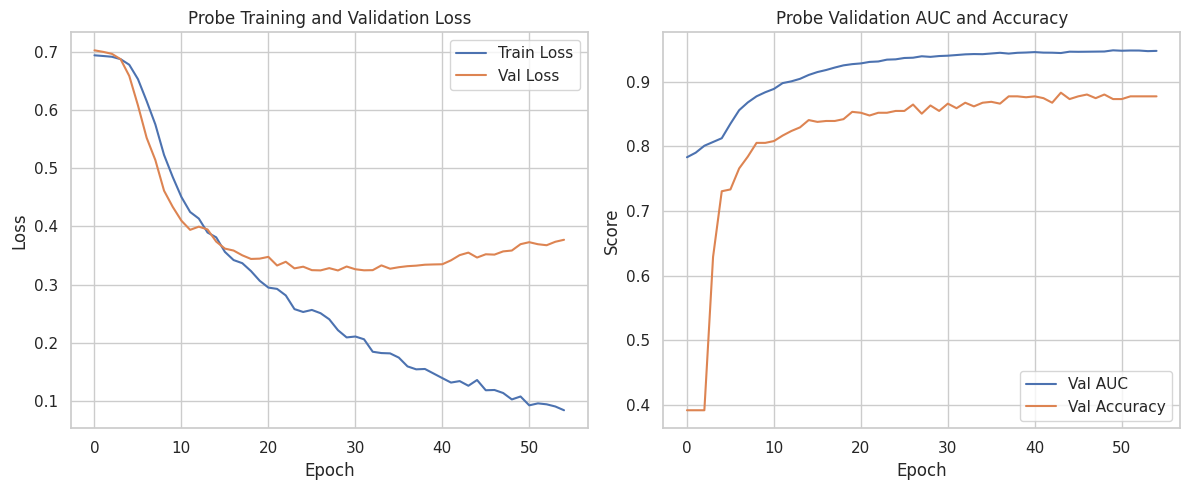
\includegraphics[width=\linewidth]{probemlp_training.png}
        \caption{Model 1 (ProbeMLP).}
    \end{subfigure}
    \begin{subfigure}{0.3\linewidth}
        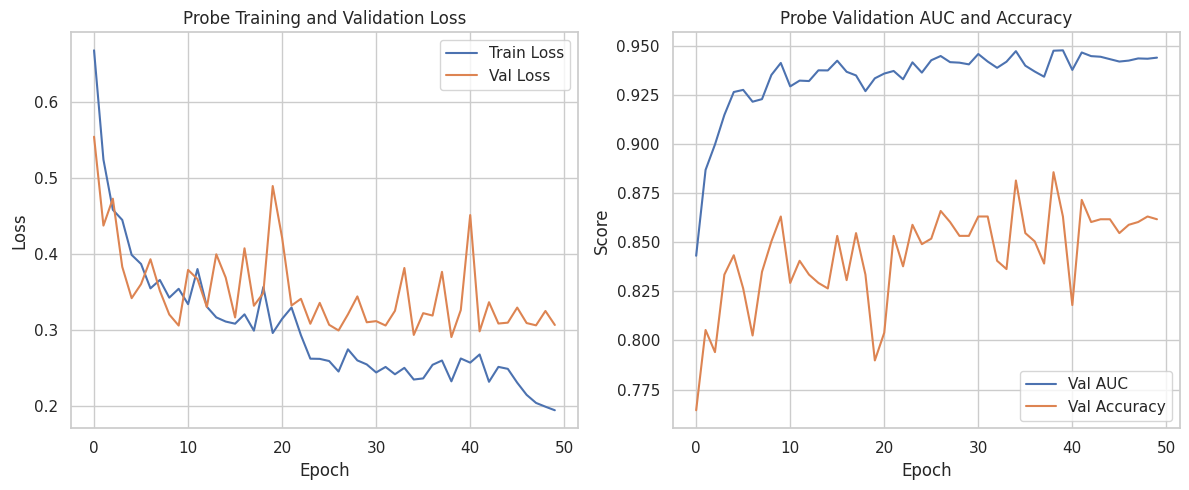
\includegraphics[width=\linewidth]{tt_training.png}
        \caption{Model 2 (Turn Transformer).}
    \end{subfigure}
    \begin{subfigure}{0.3\linewidth}
        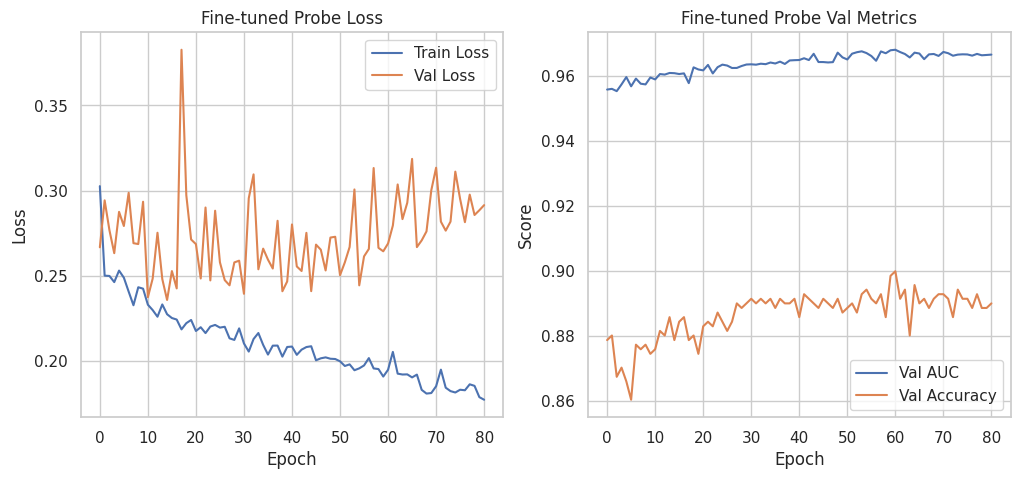
\includegraphics[width=\linewidth]{ft_tt_training.png}
        \caption{Model 3 .}
    \end{subfigure}
    \caption{Training and validation curves for all three models. Each panel shows train/val loss (left) and val AUC/accuracy (right) across epochs. Model 3 is the turn-transformer probe re-trained on the LoRA-fine-tuned encoder embeddings.}
\end{figure}

\begin{figure}[h]
    \centering
    \begin{subfigure}{0.48\linewidth}
        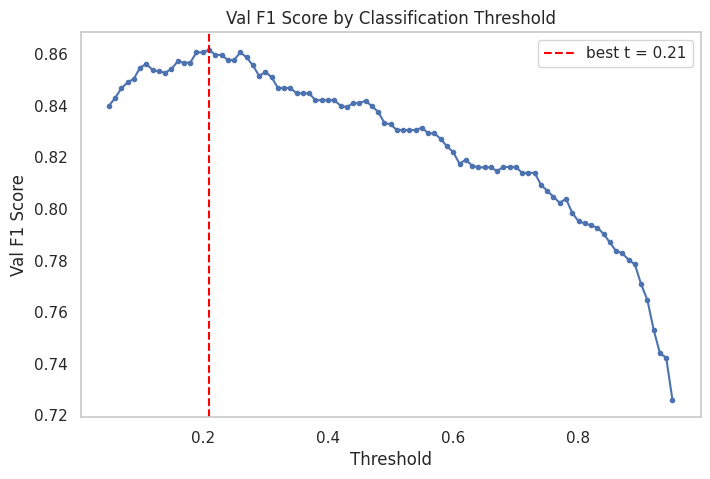
\includegraphics[width=\linewidth]{probemlp_f1_threshold.png}
        \caption{Model 1 validation F1 vs.\ threshold.}
    \end{subfigure}
    \begin{subfigure}{0.48\linewidth}
        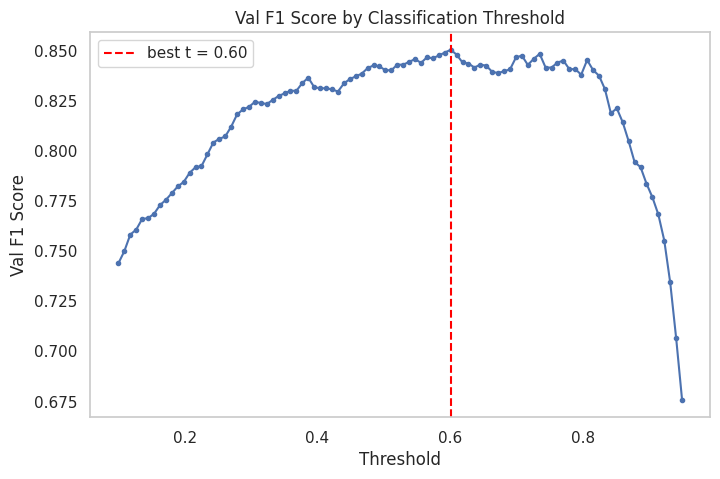
\includegraphics[width=\linewidth]{tt_f1_threshold.png}
        \caption{Model 2 validation F1 vs.\ threshold.}
    \end{subfigure}
    \caption{F1-vs-threshold curves used to select the operating threshold (0.21 for Model 1, 0.60 for Model 2; 0.45 for Model 3, not shown).}
\end{figure}

\subsection{Artifact References}

\begin{itemize}
    \item Notebook: \texttt{notebooks/MS4\_Final\_Model.ipynb} (inline code completion assisted by GitHub Copilot~\cite{copilot}).
    \item Embedding caches: \texttt{data/ds\_all\_with\_embeddings}, \texttt{data/ds\_all\_with\_turn\_embeddings}, \texttt{data/ds\_all\_with\_turn\_embeddings\_ft}.
    \item Model checkpoints: \texttt{data/probe\_final.pth}, \texttt{data/turn\_transformer\_probe\_final.pth}, \texttt{data/qwen3\_lora\_turn\_source\_invariant/}, \texttt{data/loso\_probe\_*\_final\{,\_ft\}.pth}.
\end{itemize}

%%%%%%%%%%%%%%%%%%%%%%%%%%%%%%%%%%%%%%%%%%%%%%%%%%%%%%%%%%%%


\end{document}